\documentclass[a4paper,11pt,dvipdfmx]{ujarticle}
% パッケージ
\usepackage{graphicx}
\usepackage{url}
% レイアウト指定を記述したファイルの読み込み
\input{layout}

% タイトルと氏名を変更せよ.
\title{日本におけるデジタル化の状況}
\author{G584522025 田尾優人}

\begin{document}

\maketitle %ここにタイトルが入る

% ここから本文

% を使う
% 本文(1)
%  参考文献の参照: \cite{}
%  図番号の参照: \ref{}
% を使う
% 文献データベースのキーワードは oecd と imd
% になっている.

\section{ブロードバンドの整備状況}
OECDによるブロードバンド回線の普及に関する調査\cite{oecd}によると、図\ref{fig:ランキング}に示すように、日本におけ
る100人あたりの光ファイバー回線の加入者数は29.0で、韓国、スウェーデン、ノルウェーに続いて第
4位になっている。
\begin{figure}[htbp]
    \centering
    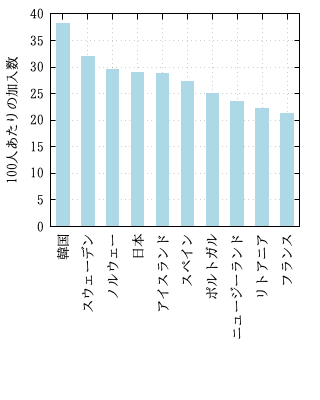
\includegraphics{fig11.png}
    \caption{光ファイバー回線の加入者数(100人あたり)}\label{fig:ランキング}
\end{figure}
% を
% \begin{figure}[htbp]
% \end{figure}
% で囲み
% \caption{}
% で図のタイトルを入れる.
% \label{}
% を使って図番号が参照できるようにする
% また,
% \centering
% で図が中央に来るようにする

% ーーー
% 節見出し(2)
\section{デジタル競争力ランキング}
国際経営開発研究所(IMD)の調査に\cite{imd}によると、日本のデジタル競争力のランキングは表\ref{tbl:デジタル}に示すよ
うに、調査対象の64カ国中、総合で28位、準備分野で27位となっている。
% 本文(2)

% 表の挿入
\begin{table}[htbp]
    \centering
    \caption{デジタル競争力ランキング(64カ国中)}
    \label{tbl:デジタル}
    \begin{tabular}{|c|c|c|}
        \hline
        国 & 総合 & 準備 \\
        \hline
        米国 & 1位 & 1位\\
        \hline 
        香港 & 2位 & 10位\\
        \hline
        スウェーデン & 3位 & 6位\\
        \hline
        デンマーク & 4位 & 2位\\
        \hline
        シンガポール & 5位 & 11位\\
        \hline
        韓国 & 12位 & 5位\\
        \hline
        中国 & 15位 & 17位\\
        \hline
        日本 & 28位 & 27位\\
        \hline
    \end{tabular}
\end{table}
% による表の記述を 
% \begin{table}[htbp]
% \end{table}
% で囲み
% \caption{}
% で表のタイトルを入れる.
% \label{}
% を使って表番号が参照できるようにする
% また,
% \centering
% で表が中央に来るようにする

% ーーー
% 見出し(3)
\section{考察}
\begin{itemize}
    \item 日本は光ファイバー回線を利用している国の中でも加入者数がかなり上位であるため、学校教育などでもインターネットを使用した教育を増やす可能性がある。
    \item アメリカはデジタル競争力ランキングが高いので、社会が日常生活においてかなりインターネットが使われていると考えられている。
\end{itemize}
% 考察
%
% \begin{itemize}
% \end{itemize}
% を使って箇条書きで記述する

% ここに参考文献が入る

%
\bibliographystyle{junsrt}
\bibliography{exercise.bib}

\end{document}